% Font size, paper type
\documentclass[12pt]{article}
% Aesthetic margins
\usepackage[margin=1in]{geometry}
% Core math packages,
% Mathtools loads amsmath, and amsmath gives basic math symbs
% Amsfonts & amssymb are misc. symbols you might need
\usepackage{mathtools, amsfonts, amssymb}
% Links in a pdf
\usepackage{hyperref}
% Use in pictures, graphs, and figures
\usepackage{graphicx}
% Header package
\usepackage{fancyhdr}
% Underlining with line breaks
\usepackage{ulem}
% Adjust accordingly given warning messages
\setlength{\headheight}{15pt}
% So we can more easily format text with pictures
\usepackage{float}
% Images and drawing graphs
\usepackage{tikz}
% Something about bits and stuff
\usepackage[T1]{fontenc}
% Set the incoding to unicode instead of ascii
\usepackage[utf8]{inputenc}
% Set the font to arial
% \usepackage{fontspec}
% \usepackage{mathspec}
% \setmainfont{Arial}
% \setmathrm{Arial}
% \setmathfont(Digits,Latin){Arial}
\usepackage{tabularx}

% Sets footer
\pagestyle{fancy}
% Removes default footer style
\fancyhf{}
\renewcommand{\headrulewidth}{0pt}


\rhead{
\thepage{}
}

% Makes links look more appealing
\hypersetup{
colorlinks=true,
linkcolor=blue,
filecolor=magenta,      
urlcolor=cyan,
}

% \usepackage{indentfirst}

\begin{document}
\title{Young's Experiment Lab Conclusion (ADD UNCERTAINTY TO GRAPH)}
\author{by Shengdong Li}
\date{28 September 2021}
\maketitle

\section{Research Question}

What happened in Young's Double-Slit Experiment?

\section{Purpose}

The purpose of Young's Experiment is to gain a better understanding of double-slit diffraction by seeing and interacting with an example in real life.

\section{Variable and Explanations}

In this lab, all variables were kept constant.

\begin{itemize}
	\item \textbf{Distance between slits} The distance between slits is of vital importance, because if the slit is too big or too small relative to the wavelength of the light diffraction will not occur at all. As distance between the slits increases, the wavelength will increase, and as distance between the slit decreases, the wavelength of light will decrease.
	\item \textbf{Distance from node to node} The distance from node to node of the light diffracting through the slit. This will be measured via ruler, when the number of bright fringes between the paper slips are even. However, as this variable increases, the wavelength won't unconditionally go up because the order of the fringes will also go up.
	\item \textbf{The order of the fringes} The order of fringes is the number of dark and light fringes. It will be measured by counting the number of bright fringes between paper slips via eye. As the order goes up, the wavelength decreases, though the distance from node to node is tied to the order of the fringes.
	\item \textbf{Distance between the slit and the screen} The distance between the slip and light from the lamp will be measured via a tape measure going from the slit directly to the light. As the distance from the slit to the fringe increases, the wavelength may or may not go up, since the distance between nodes is tied to the light.
\end{itemize}

\subsection{Sketch Defining the Variables Used}

\begin{figure}[H]
	\centering
	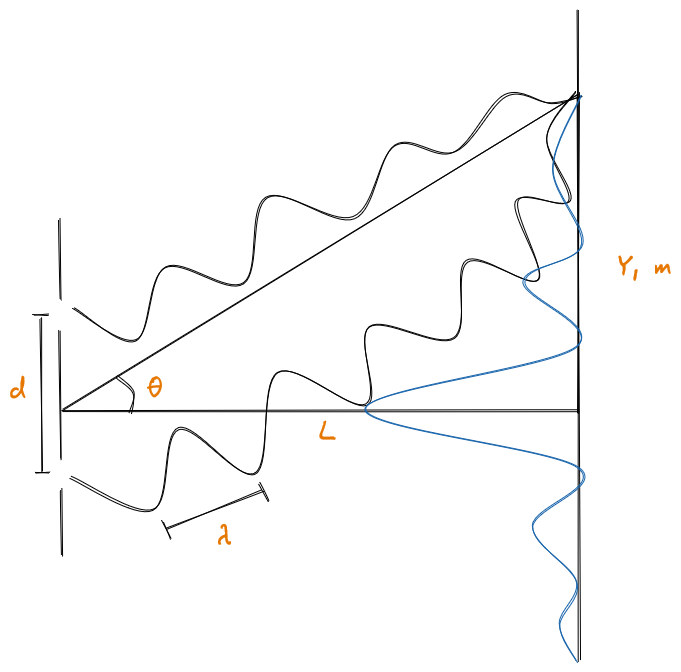
\includegraphics[scale=0.7]{sketch.png}
	\caption{Sketch of double-slit diffraction}
\end{figure}

\section{Materials List}

\begin{itemize}
	\item 1 light
	\item 1 double slit with a distance of $0.176\ m$ between both slits
	\item 1 tape measure
	\item 1 ruler
	\item 2 wide and lengthy paper slips
	\item 1 slit stand
\end{itemize}

\section{Procedure}

\begin{enumerate}
	\item Set the slit stand on a flat surface
	\item Fix the slit on the slit stand
	\item Measure 4 meters out from the slit
	\item Place the light at an even level to the stand
	\item Put a meter stick behind the light
	\item Turn on the light
	\item Look through the slits that are $0.176\ m$ apart
	\item From the center of the diffraction pattern, put 1 slip of paper on the closest dark fringe to the left
	\item Repeat the previous step except put the paper slip to the right
	\item Measure the distance between the two slips
	\item Count the number of bright fringes between the two slips
\end{enumerate}

\section{Raw Data Table}

\begin{table}[H]
	\def\arraystretch{1.5}
	\resizebox{\textwidth}{!}{\begin{tabular}{lllll}
			\hline
			Distance slit-slit (m) & Distance n-n (m) & Order & Distance light-screen (m) \\
			\hline
			0.000176               & 0.08             & 3     & 4.14
		\end{tabular}}
\end{table}

\section{Sample Calculations}
\textbf{Calculating the wavelength of the light}
\begin{align*}
	\intertext{We measured a distance of \(0.08 m\) between the two paper slips, but we divide it by 2, since \(y\) only measures the distance from the center to the bright/dark fringe on one side}
	y           & =\frac{0.08\ m}{2}=0.04\ m                       \\
	\intertext{Distance between the slits}
	d           & =0.176\ mm\cdot\frac{1\ m}{1000\ mm}=0.000176\ m \\
	\intertext{Order}
	m           & =3                                               \\
	\intertext{Distance from slit to screen}
	L           & =4.14\ m                                         \\
	\intertext{We have following formula}
	d\sin\theta & =m\lambda                                        \\
	\intertext{Where \(d\) is the distance between the two slits, \(\theta\) is the angle of the diffracted bean of light, \(m\) is the order of interference, and \(theta\) is the wavelenght of light.}
	\intertext{For small angles, }
	\sin\theta  & =\tan\theta=\theta                               \\
	\intertext{So we can replace \(\sin\theta\) with \(\theta\) }
	d\theta     & =m\lambda
\end{align*}
And since \(\tan\theta=\theta\), and \(\tan\) is opposite over adjacent in the following triangle:
\begin{figure}[H]
	\begin{center}
		\begin{tikzpicture}
			\draw (0,0) node[anchor=north]{}
			-- (2,0) node[below]{$L$}
			-- (4,0) node[anchor=north]{}
			-- (4,2) node[right]{$y$}
			-- (4,4) node[anchor=south]{}
			-- cycle;
		\end{tikzpicture}
	\end{center}
\end{figure}
\begin{align*}
	\intertext{We can substitute \(\theta\) with the meaning of \(\tan\)}
	\theta       & =\frac{y}{L}                                                                             \\
	\intertext{This gives us the following}
	d\frac{y}{L} & =m\lambda                                                                                \\
	\intertext{We can divide both sides by \(m\) to get}
	\lambda      & =\frac{dy}{mL}                                                                           \\
	\intertext{We plugin all our values in the table to get}
	\lambda      & =\frac{\left(0.000176\ m\right)\left(0.04\ m\right)}{\left(4.14\ m\right)\left(3\right)} \\
	\Aboxed{     & =5.67\cdot10^{-7}\ m}
\end{align*}

\section{Calculated Data Table}

\begin{table}[H]
	\def\arraystretch{1.5}
	\resizebox{\textwidth}{!}{\begin{tabular}{lllll}
			\hline
			Distance slit-slit (m) & Distance n-n (m) & Order & Distance light-screen (m) & Wavelength of Light (m) \\
			\hline
			0.000176               & 0.08             & 3     & 4.14                      & \(5.67 \cdot 10^{-7}\)
		\end{tabular}}
\end{table}

\section{Analysis (Answering the two questions)}


\begin{itemize}
	\item \textbf{What do you observe happening to the diffraction pattern? Describe how the difraction pattern changes as the slit width gets narrower}
	      \subitem As the slit width gets narrower, the distance between the individual dark and light fringes gets wider, and so the diffraction pattern becomes more and more distinguishible.
	\item \textbf{Look through your slitfilm at a white bulb in the clasroom. If you look very carefully at the nodal lines, notice that the bars towards the ends are slightly colored. Why do you think these are colored?}
	      \subitem The bars towards the ends are slightly colored, since the different 'colors' of visible light have different wavelengths. And as the distance from the center increses, closer to the left and right fringes, this difference in wavelength between the different colors becomes visible.
\end{itemize}

\section{Conclusion}
The distance the car gravity car travels is constant as the mass of the car increases. This is because, while the line of best fit has a slightly positive relationship, its slope is very low at \(0.04\) and the points fluctuate around and have high uncertainty. This is further supported by the fact that one gradient line has a slope of \(0\). At a mass of \(116g\), the car traveled an average distance of around \(171.5cm\), but from masses \(145-165\) the distance the car traveled was slightly less than the beginning, an average of \(166cm\). Only at a mass of \(174g\) did the car begin to have a slightly increased average distance of \(172cm\), but this was almost the same distance traveled as the very first trial. This goes against the original hypothesis that the car would travel less distance as mass increases. This nondifference can be explained by Newton's First and Second Laws of motion.

Upon closer inspection of the forces at work, it can be seen that there are two distinct phases of forces acting on the gravity car: when the car goes down the ramp, and when the car is traveling on the ground after it has accelerated on the ramp. On the ramp, there is a greater force pushing on the gravity car with more Scrabble pieces, since the \(x\) component of the weight force is dependent on mass \(w_x = w\sin(\theta)\). But the thing is, even though there is a bigger force acting on the bigger car, the smaller car and the bigger car both move down the ramp at the same speed. Newton's Second law of motion states acceleration is proportional to force but inversely proportional to mass, such that that \(a=\frac{F}{m}\). When the weight component is substituted into the equation, in the resulting equation the masses cancel.
\begin{align*}
	\sum F_x  & = w\sin(\theta)            \\
	ma        & = mg\sin(\theta)           \\
	a         & = \frac{mg\sin(\theta)}{m} \\
	\Aboxed{a & =g\sin(\theta)}
\end{align*}
A greater force or push does not equal greater acceleration in this case. Both heavy and light cars reach the bottom of the ramp at the same speed.

Then, when the gravity car is moving on level ground, the only horizontal force is kinetic friction pulling the car back.
\begin{align*}
	\sum F_{x} & =-F_{k}            \\
	           & =-u_{k}\cdot F_{N} \\
	           & =-u_{k}\cdot mg
\end{align*}
In this case, a heavier car would result in a greater kinetic friction force backward. But if Newton's second law is applied again it can be seen that the decrease in acceleration of both cars is equal once again
\begin{align*}
	\sum F_{x} & =ma             \\
	ma         & =-u_{k}\cdot mg \\
	\Aboxed{a  & =-u_{k}\cdot g}
\end{align*}
It all goes back to Newton's first law of motion, that heavier objects have more inertia and so require more forces to both stop and move.

\section{Evaluation of Strengths and Weaknesses}
Because this was an experiment done at home due to quarantine, there were many limitations and possible sources of error in the experiment. One such source of error was the horizontal positioning of the gravity car on the ramp. While the height of the car on the ramp was part of the control variables, the width of the ramp made it much harder to position the car correctly horizontally every time. While by itself this might not have been much of an issue, the other problem was that the floorboards were uneven. Sometimes, if the car was positioned a couple of centimeters to the left it would bump into more crevices in the floorboards, resulting in a lower distance traveled. While the material of the floor should've stayed the same, it ultimately could've caused the large uncertainty and fluctuations in the data table. Another source of error was that the axle of the car was partially broken, so it would sometimes veer slightly to the right. This would've resulted in some of the measured distances traveled being lower than they should've been.

\section{Improvements}
Many things could be done in the future to address the car issues. One is to buy a new toy car that isn't broken, so it doesn't veer to the right. To address the issue of the horizontal alignment of the car causing the uneven material of the wooden floorboards to have an impact on the garage floor could've been used. Another thing that could be done is to mark a specific spot on the ramp to always position the car correctly on the ramp.
\end{document}
